\clearpage
\markboth{Problem 5}{Problem 5: Part 2}

\textbf{Problem Statement:} Implement and analyze the Ridders' method for solving the equation $f(x) = 0$. For guidance, you might wish to read the Wikipedia page on the Ridders' method. Also feel free to consult other sources.

\subsection*{Brief Description of the method}

Given the initial bracketing interval $[x_0, x_2]$, containing \textbf{one} solution, and such that $f(x_0)$ and $f(x_2)$ have opposite signs, compute the midpoint $x_1 = (x_0 + x_2)/2$. Then define a new function $h(x) = f(x)e^{ax}$. Find the parameter $a$ that ensures $h(x_1) = \frac{1}{2}(h(x_0) + h(x_2))$. Then define $x_3$ as the $x$-intercept of the line passing through $(x_0, h(x_0))$ and $(x_2, h(x_2))$. Use $x_3$ as one of the endpoints of the next interval bracketing the solution. The other endpoint is $x_1$ if $f(x_1)f(x_3) < 0$. Otherwise, choose either $x_0$ or $x_2$ based on the requirement that the sign of $f(x)$ at the chosen point must be opposite to the sign of $f(x_3)$. Continue until the desired accuracy is reached.

\subsection*{Part 2}
\addcontentsline{toc}{subsection}{Problem 5.2}

Work out a formula for $x_3$ in detail.

\noindent\rule{\textwidth}{0.4pt}

\vspace{1em}

\textbf{Solution:}

\begin{center}
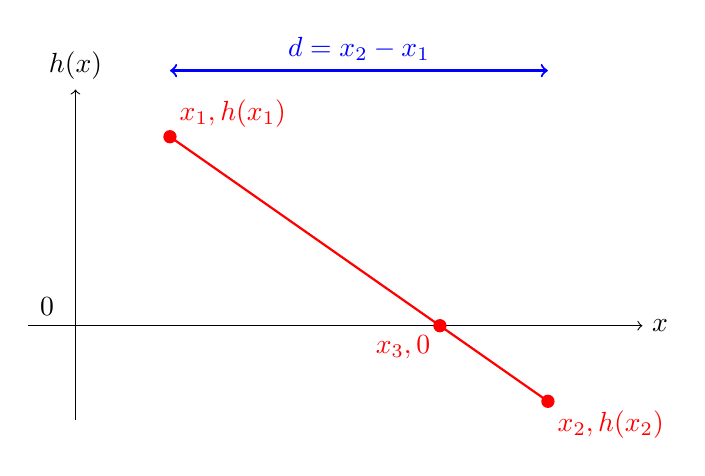
\begin{tikzpicture}[scale=1.2]
    % Draw axes
    \draw[->] (0,-1) -- (0,2.5) node[above] {$h(x)$};
    \draw[->] (-0.5,0) -- (6,0) node[right] {$x$};
    
    % Define points: x1 at position 1 with positive h, x2 at position 5 with negative h
    % Line passing through (1, 2) and (5, -0.8) intersects x-axis at x3
    % Calculate x3: (2 - 0)/(2 - (-0.8)) = 2/2.8, so x3 = 1 + (2/2.8)*4 ≈ 3.857
    
    % Draw the line through (x1, h1) and (x2, h2)
    \draw[red, thick] (1,2) -- (5,-0.8);
    
    % Draw distance d between x1 and x2
    \draw[<->, blue, thick] (1,2.7) -- (5,2.7) node[midway, above] {$d = x_2 - x_1$};
    
    % Mark points
    \fill[red] (1,2) circle (2pt) node[above right] {$x_1, h(x_1)$};
    \fill[red] (5,-0.8) circle (2pt) node[below right] {$x_2, h(x_2)$};
    \fill[red] (3.857,0) circle (2pt) node[below left] {$x_3, 0$};
    
    % Label "0" on y-axis
    \node at (-0.3,0.2) {$0$};
\end{tikzpicture}
\end{center}

\vspace{0.5em}

From the diagram, we want to find $x_3$, the x-intercept of the line passing through $(x_1, h(x_1))$ and $(x_2, h(x_2))$.

Let $h_1 = h(x_1)$ and $h_2 = h(x_2)$. The slope of the line is:
\[
    m = \frac{h(x_1) - h(x_2)}{x_1 - x_2} = \frac{h_1 - h_2}{x_1 - x_2}
\]

The equation of the line passing through $(x_1, h_1)$ with slope $m$ is:
\[
    h(x) - h_1 = m(x - x_1)
\]

To find $x_3$, set $h(x_3) = 0$:
\[
    0 = h_1 + m(x_3 - x_1)
\]

Solving for $x_3$:
\[
    m(x_3 - x_1) = -h_1
\]
\[
    x_3 - x_1 = -\frac{h_1}{m}
\]
\[
    x_3 = x_1 - \frac{h_1}{m}
\]

Substitute the expression for $m$:
\[
    x_3 = x_1 - \frac{h_1}{\frac{h_1 - h_2}{x_1 - x_2}}
\]
\[
    x_3 = x_1 - \frac{h_1(x_1 - x_2)}{h_1 - h_2}
\]

Now, using $d/2 = x_2 - x_1$, we have:

\[
    \boxed{x_3 = x_1 + \frac{d}{2} \cdot \frac{1}{1 - h_2/h_1}}
\]

Or equivalently:
\[
    \boxed{x_3 = \frac{x_1 h_2 - x_2 h_1}{h_2 - h_1}}
\]

\vspace{2em}
\noindent\rule{\textwidth}{0.4pt}
